% Standalone pgfplots figure -- compile with pdflatex/lualatex, or
% \input{} into a document that loads \usepackage{pgfplots}.
% Surface code d=11 memory_X, filtered-X p-bit decode. LER per cycle (=LER_shot/11).
\documentclass[tikz,border=3mm]{standalone}
\usepackage{pgfplots}
\pgfplotsset{compat=1.17}
\begin{document}
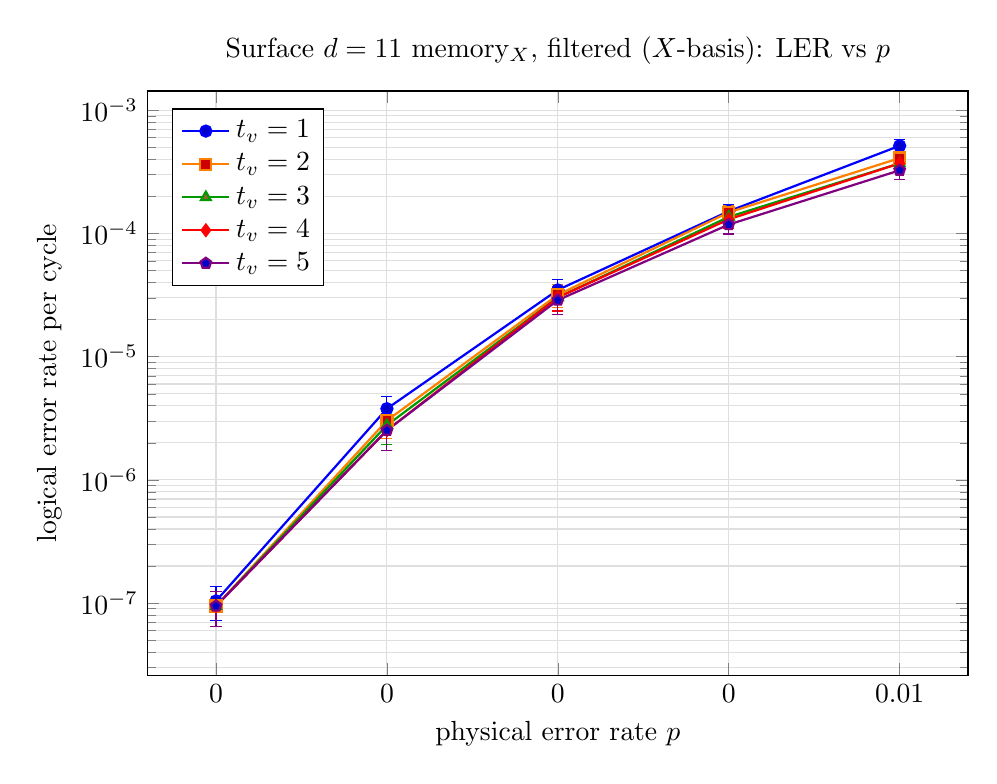
\begin{tikzpicture}
\begin{semilogyaxis}[
    width=12cm, height=9cm,
    xlabel={physical error rate $p$},
    ylabel={logical error rate per cycle},
    title={Surface $d=11$ memory$_X$, filtered ($X$-basis): LER vs $p$},
    xtick={0.001,0.002,0.003,0.004,0.005},
    scaled x ticks=false, x tick label style={/pgf/number format/fixed},
    grid=both, grid style={gray!25},
    legend pos=north west, legend cell align=left,
    mark options={solid}, every axis plot/.append style={thick},
]
\addplot+[color=blue, mark=*, error bars/.cd, y dir=both, y explicit]
    coordinates {(0.001, 1.0418e-07) +- (0, 3.1818e-08) (0.002, 3.7882e-06) +- (0, 1.0000e-06) (0.003, 3.4845e-05) +- (0, 7.2727e-06) (0.004, 1.5155e-04) +- (0, 2.1818e-05) (0.005, 5.1518e-04) +- (0, 6.2727e-05)};
\addlegendentry{$t_v=1$}
\addplot+[color=orange, mark=square*, error bars/.cd, y dir=both, y explicit]
    coordinates {(0.001, 9.4727e-08) +- (0, 3.0000e-08) (0.002, 3.0300e-06) +- (0, 8.7273e-07) (0.003, 3.1818e-05) +- (0, 6.9091e-06) (0.004, 1.4845e-04) +- (0, 2.0909e-05) (0.005, 4.0909e-04) +- (0, 5.5455e-05)};
\addlegendentry{$t_v=2$}
\addplot+[color=green!60!black, mark=triangle*, error bars/.cd, y dir=both, y explicit]
    coordinates {(0.001, 9.4727e-08) +- (0, 3.0000e-08) (0.002, 2.7782e-06) +- (0, 8.3636e-07) (0.003, 3.0300e-05) +- (0, 6.8182e-06) (0.004, 1.3636e-04) +- (0, 2.0000e-05) (0.005, 3.7118e-04) +- (0, 5.2727e-05)};
\addlegendentry{$t_v=3$}
\addplot+[color=red, mark=diamond*, error bars/.cd, y dir=both, y explicit]
    coordinates {(0.001, 9.4727e-08) +- (0, 3.0000e-08) (0.002, 2.5255e-06) +- (0, 8.0000e-07) (0.003, 3.0300e-05) +- (0, 6.8182e-06) (0.004, 1.3027e-04) +- (0, 2.0000e-05) (0.005, 3.7118e-04) +- (0, 5.2727e-05)};
\addlegendentry{$t_v=4$}
\addplot+[color=violet, mark=pentagon*, error bars/.cd, y dir=both, y explicit]
    coordinates {(0.001, 9.4727e-08) +- (0, 3.0000e-08) (0.002, 2.5255e-06) +- (0, 8.0000e-07) (0.003, 2.8791e-05) +- (0, 6.6364e-06) (0.004, 1.1818e-04) +- (0, 1.9091e-05) (0.005, 3.2573e-04) +- (0, 5.0000e-05)};
\addlegendentry{$t_v=5$}
\end{semilogyaxis}
\end{tikzpicture}
\end{document}
